\chapter{Integração}

Nos capítulos anteriores foi apresentado o detalhe de cada subsistema do projeto, neste será detalhado o processo de integração de cada subsistema.

\section{Software - Eletrônica}

Sendo a principal interface entre o usuário da bancada e o motor o SBAM possui a seguinte interface inicial.
Onde o usuário deverá fazer um login antes de iniciar a	 análise. 

\begin{figure}[h!]
	\centering
	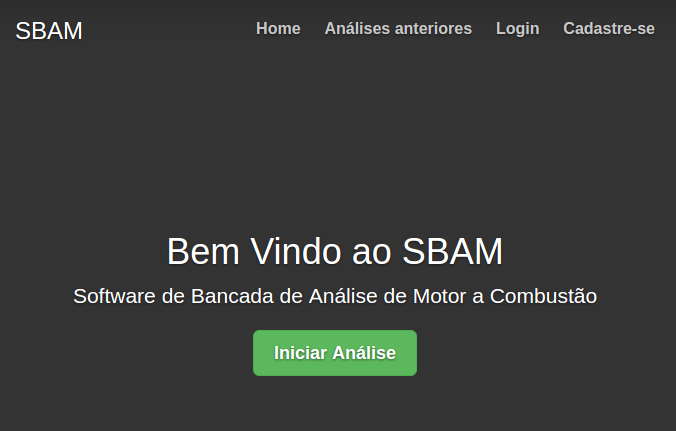
\includegraphics[keepaspectratio=true,scale= 0.7]{figuras/SBTM-TelaInicial.png}
	\caption{Tela inicial SBTM.}
	\label{telainicialSbtm}
\end{figure}

Após a realização da autenticação pode-se realizar o acionamento do motor e o usuário da bancada é redirecionado para a tela da da figura \ref{acionamentoDoMotor}, o detalhamento do processo de integração da parte de controle é apresentado nas subseções seguintes.

\subsection{Controle}

Para realização do módulo de controle o usuário deverá acionar o motor, selecionando o botão apresentado na figura \ref{acionamentoDoMotor}.

\begin{figure}[h!]
	\centering
	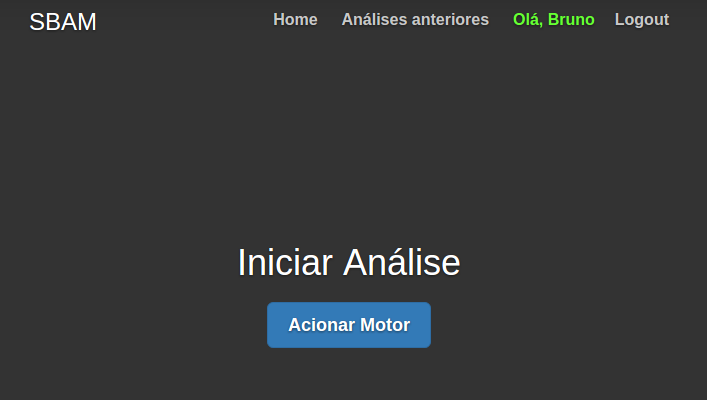
\includegraphics[keepaspectratio=true,scale= 0.7]{figuras/acionarMotor.png}
	\caption{Tela de acionamento do motor.}
	\label{acionamentoDoMotor}
\end{figure}

Isso faz com que a comunicação via protocolo TCP seja realizada entre a aplicação e a raspberry, onde a aplicação envia uma mensagem "on" para a raspberry seguindo o trecho de código em python. 

\textbf{Aplicação SBAM - Cliente:}

\begin{lstlisting}
def sendMessage():

	TCP_IP = '<ip_raspberry>'
	TCP_PORT = <porta>
	BUFFER_SIZE = 2
	MESSAGE = "on"

	s = socket.socket(socket.AF_INET, socket.SOCK_STREAM)
	s.connect((TCP_IP, TCP_PORT))
	s.send(MESSAGE)
	data = s.recv(BUFFER_SIZE)
	s.close()
\end{lstlisting}

\pagebreak

Já na raspberry(servidor) o trecho de código em linguagem C apresentado abaixo, recebe a mensagem disparada pelo SBAM (cliente), e envia uma mensagem de volta para o cliente.

\textbf{Raspberry - Servidor:}

\begin{lstlisting}
while( (read_size = recv(client_sock , client_message , 2000 , 0)) > 0 )
{
	
	write(client_sock , client_message , strlen(client_message));
}
\end{lstlisting}
 
Seguindo no fluxo de comunicação a raspberry envia o valor 85 para a MSP-430 estabelecendo a comunicação entre eles, então a função para o acionamento do motor é executada fazendo que um pino de uma porta GPIO altere seu estado lógico de 0 para 1, este pino possui conexão direta com o relê de partida do motor, fazendo então, que a modificação do estado acione o motor.

\subsection{Aquisição}

Para a implementação do modulo de aquisição da aplicação foi modelado no banco um tipo genérico para cada tipo de sensor como temperatura, pressão e RPM, onde são armazenados todas as informações dos sensores. Essas informações estão atreladas as informações da bacada de teste (usuário da bancada, data de execução da análise e uma descrição). As informações da parte de aquisição só poderão ser consultadas se antes o usuário estiver realizado o acionamento do motor e inicializado a analise. 
As informações advindas dos sensores, são processadas na raspberry e enviadas para a aplicação. 

\section{Integração Estrutural}

\begin{figure}[h!]
	\centering
	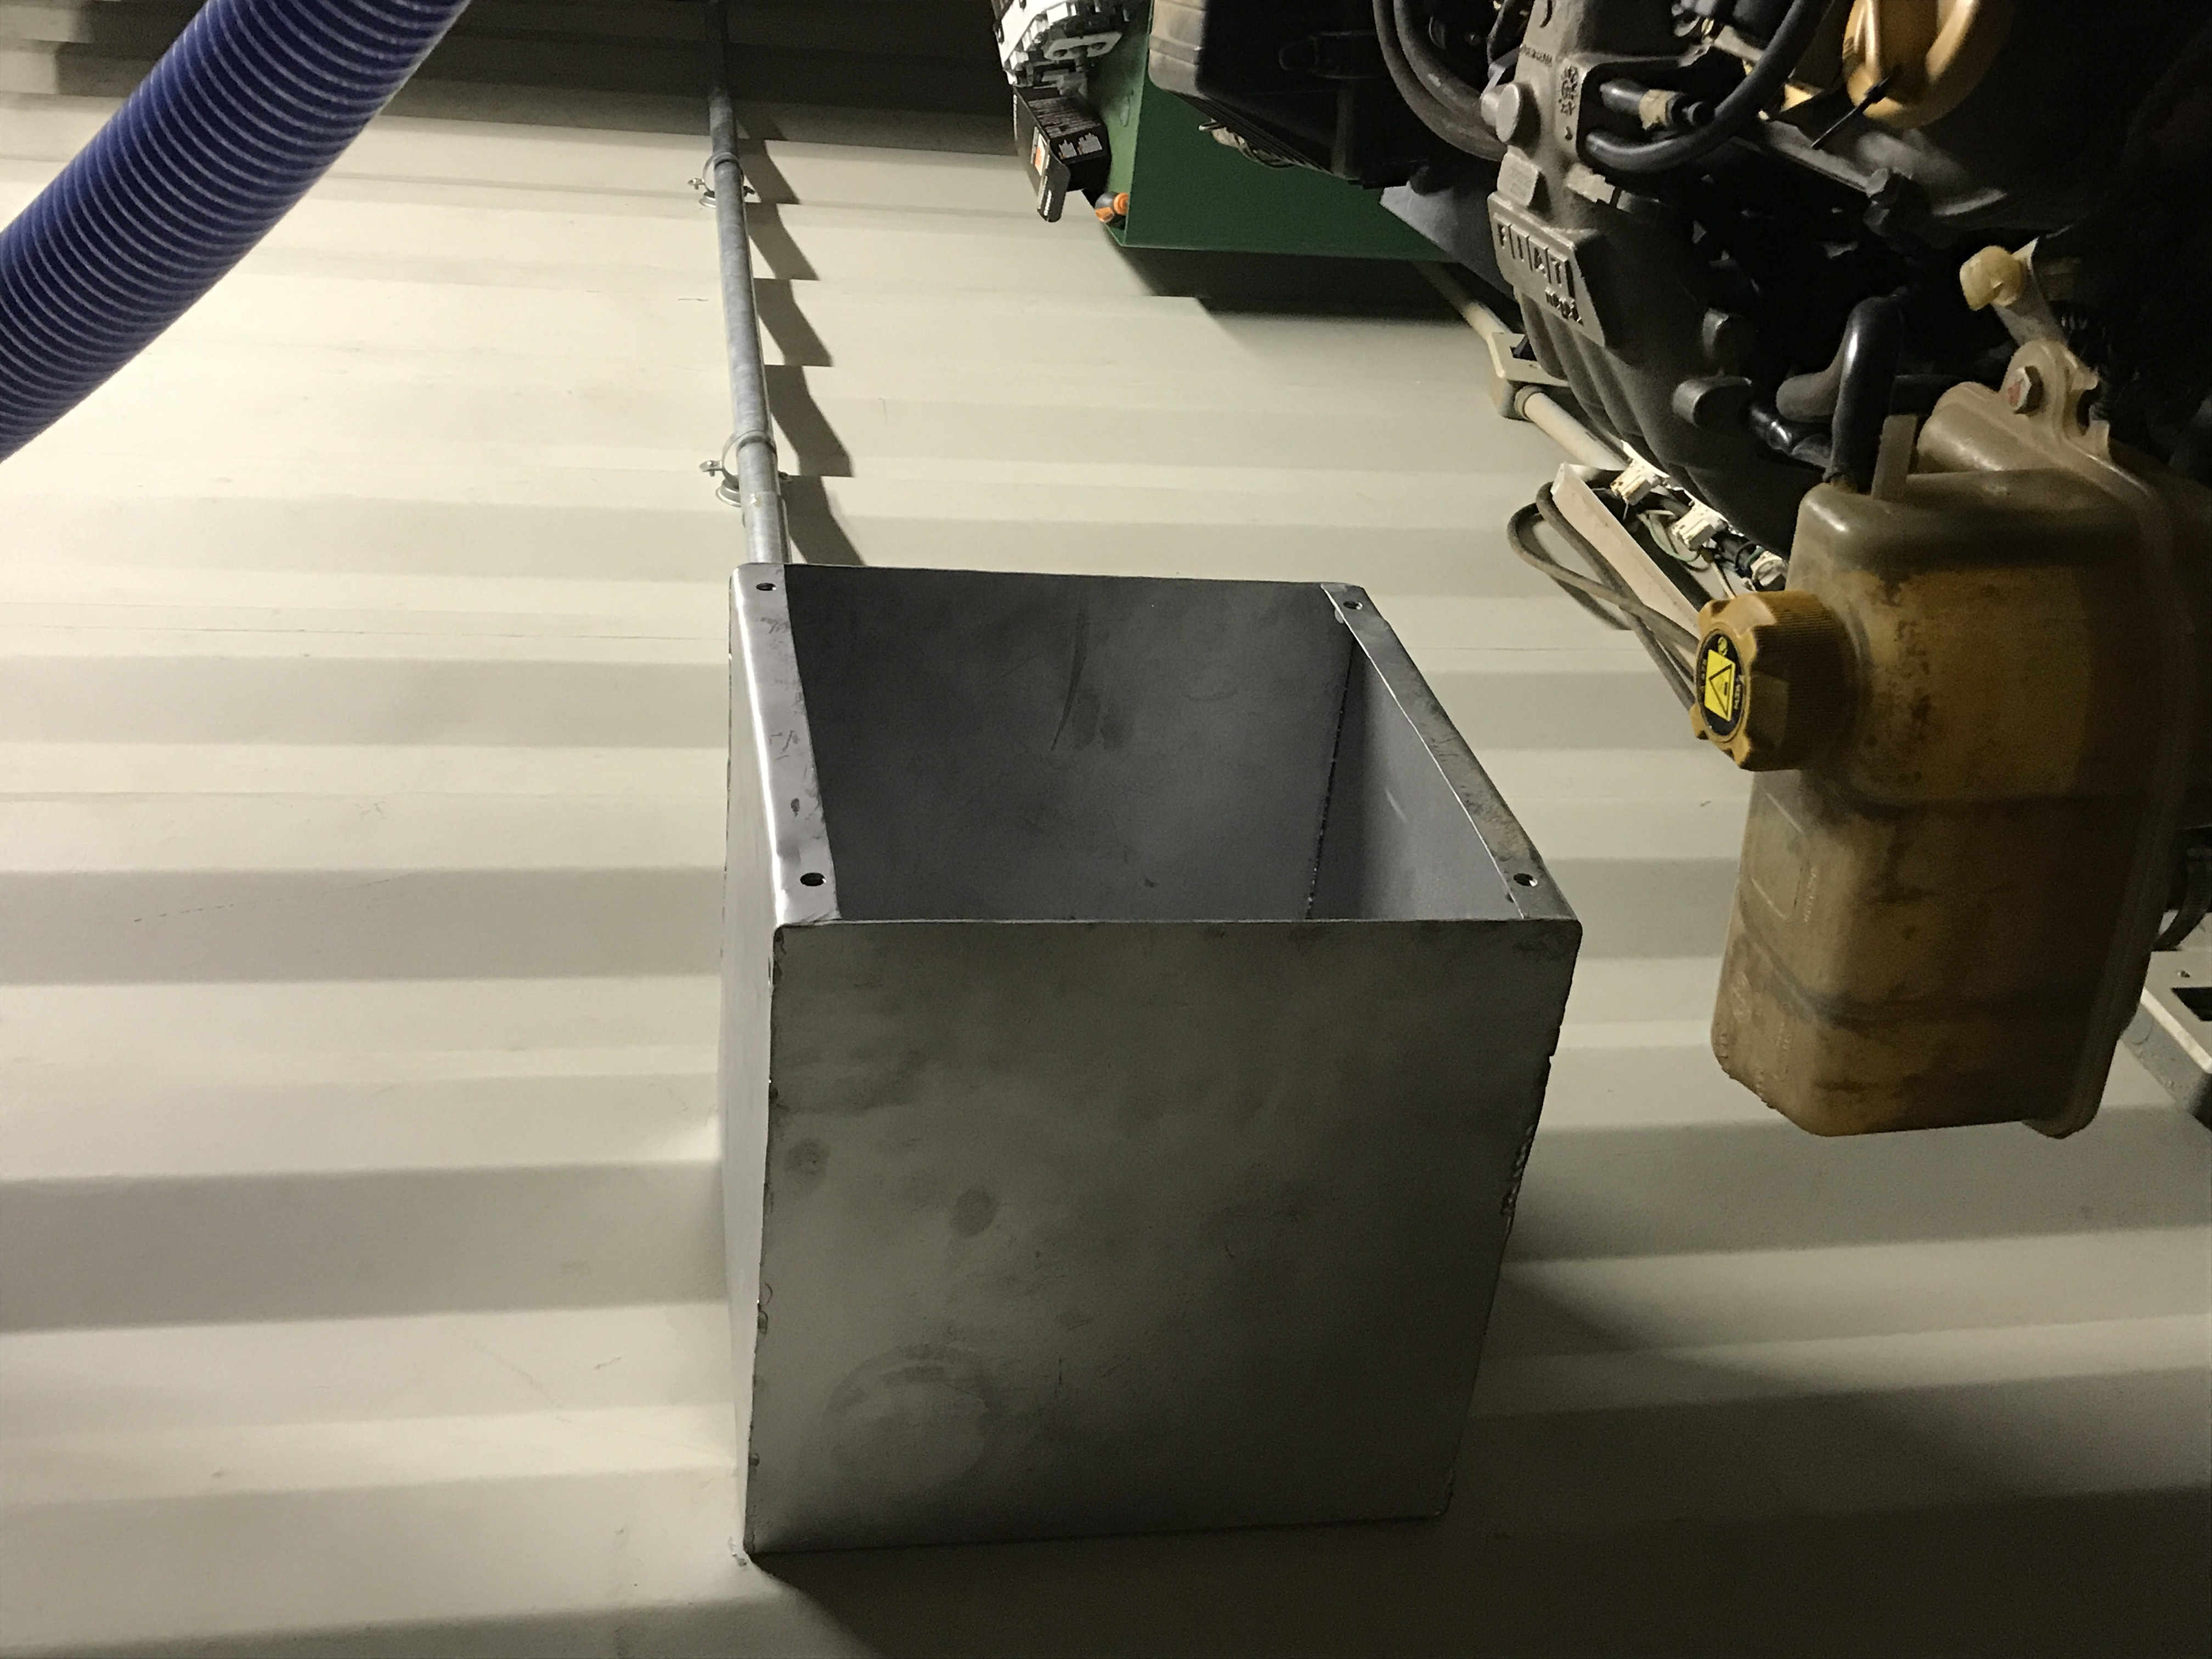
\includegraphics[angle=270,keepaspectratio=true,scale= 0.09]{figuras/caixaDeAcoplamentoDosComponentesEletronicos.JPG}
	\caption{Caixa de acoplamento dos componentes do motor}
	\label{caixaDeAcoplamento}
\end{figure}


\begin{figure}[h!]
	\centering
	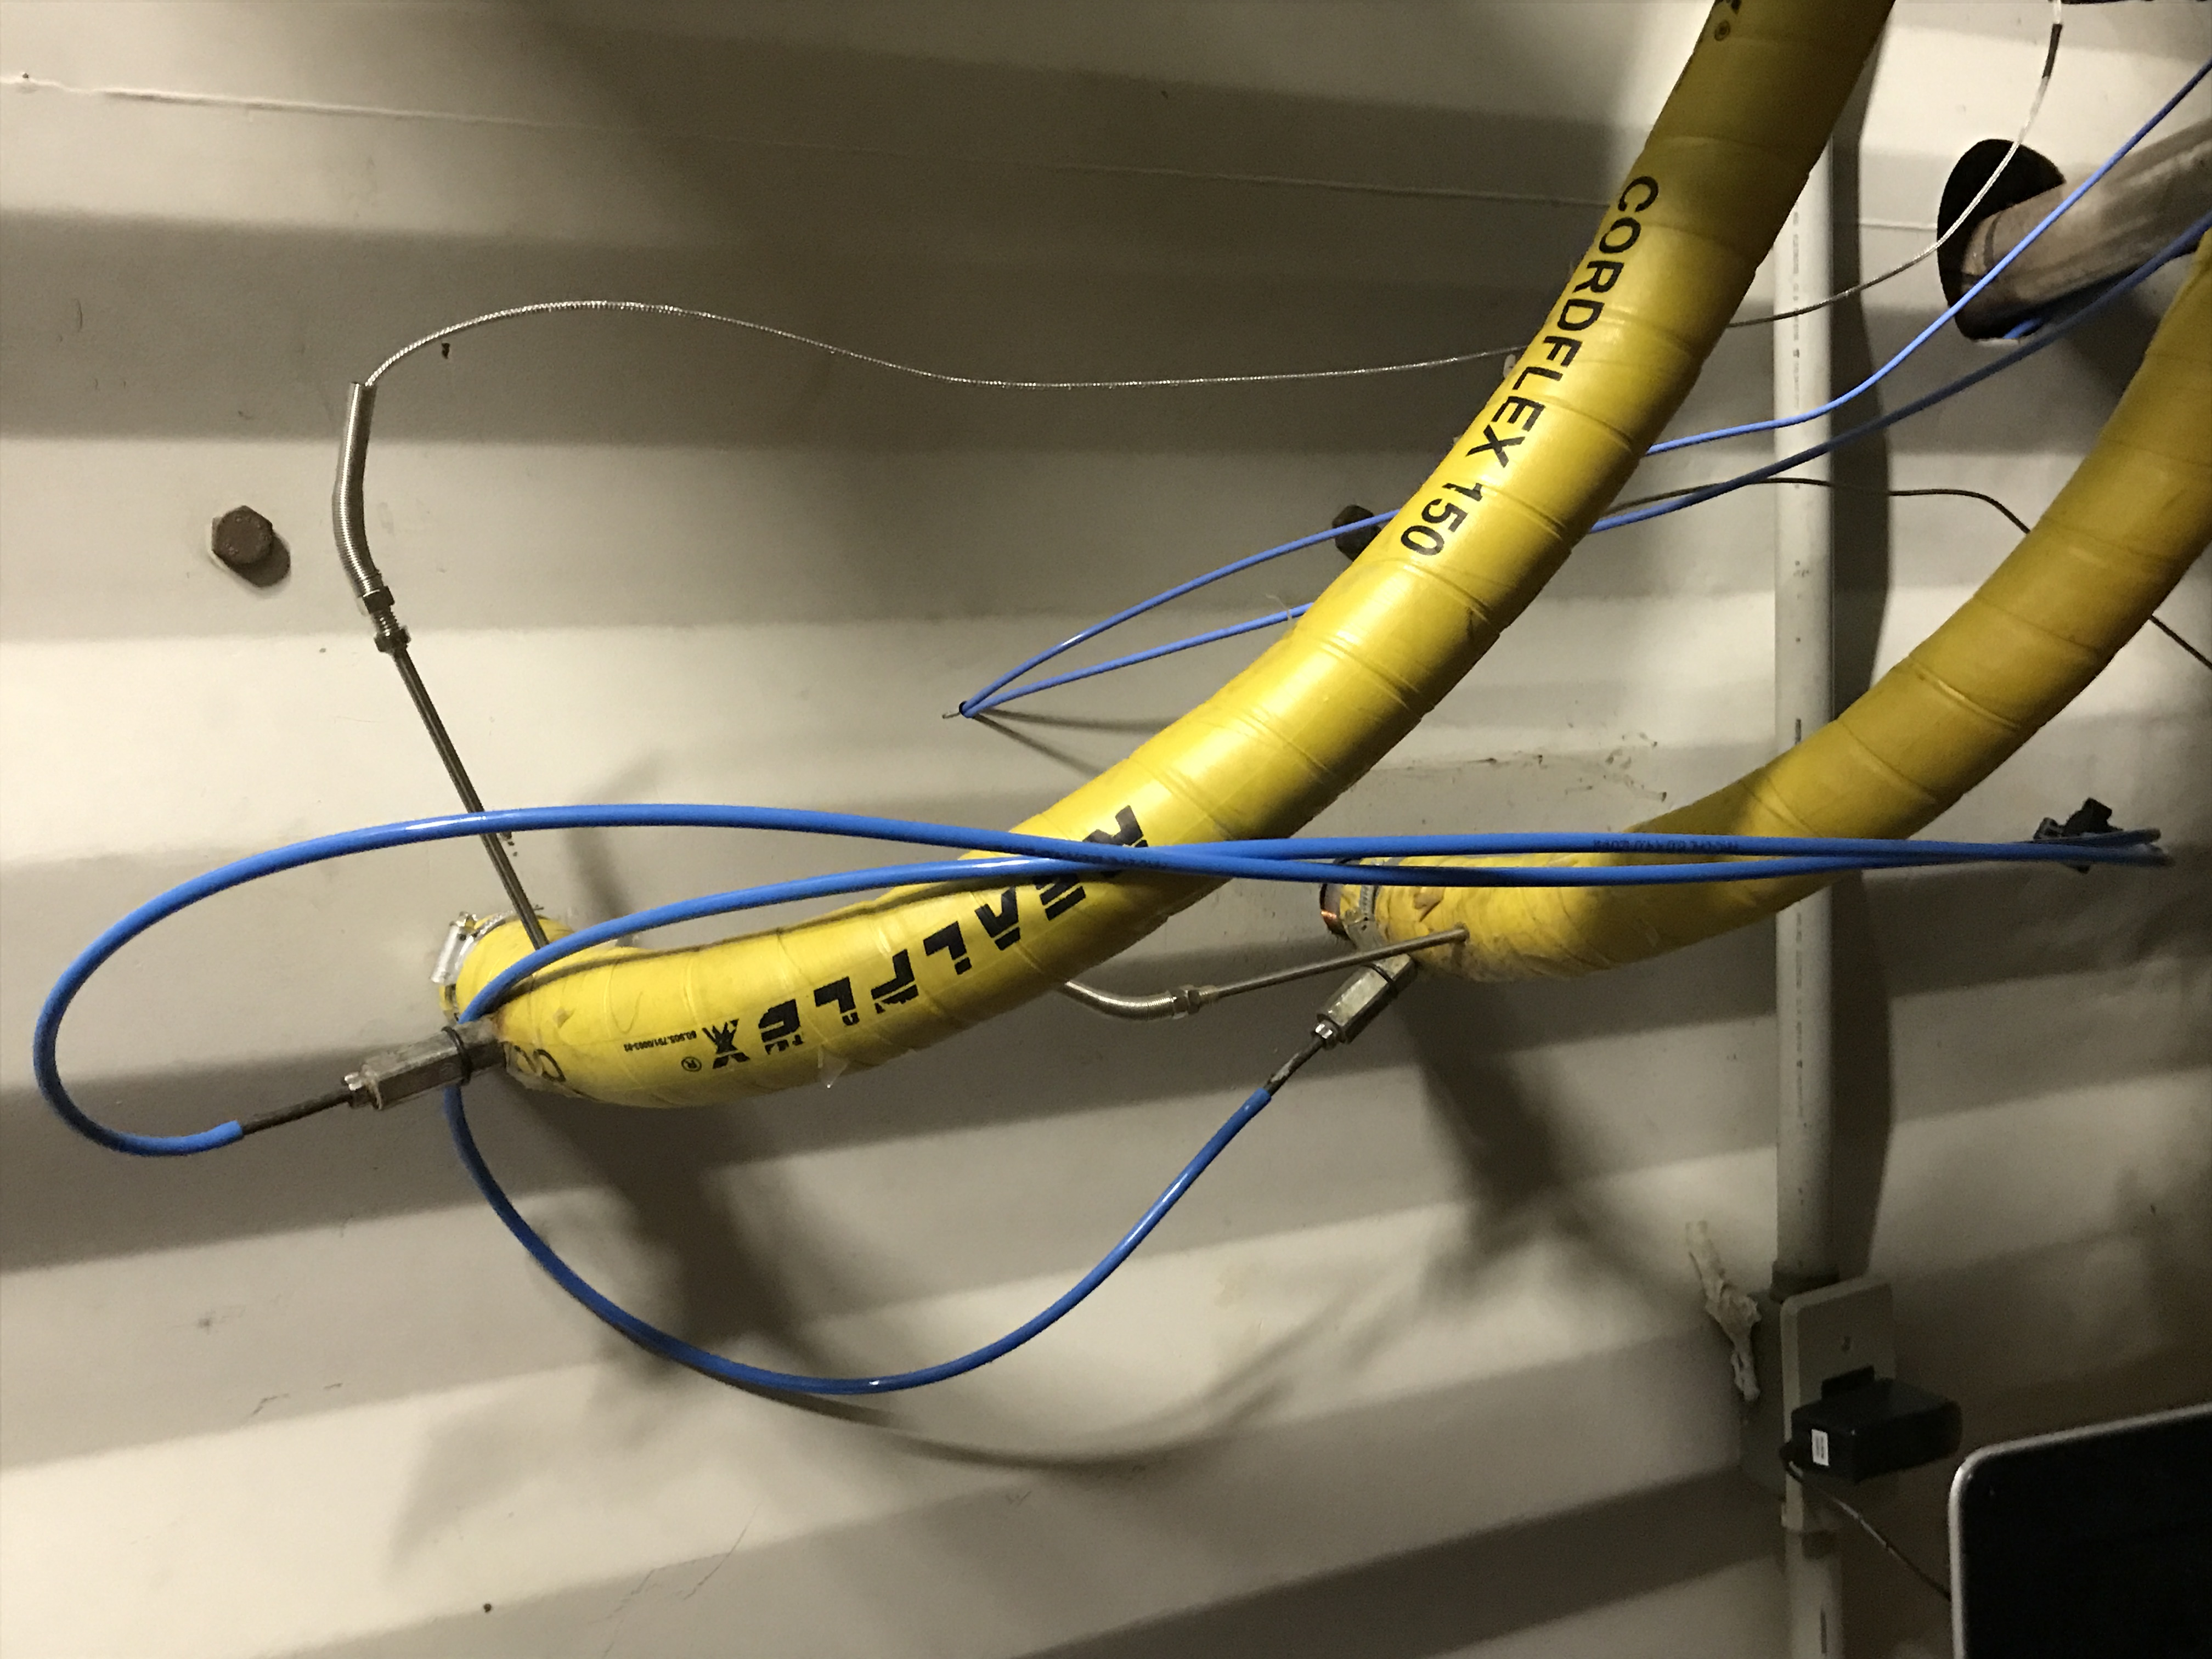
\includegraphics[angle=270,keepaspectratio=true,scale= 0.09]{figuras/AcoplamentoDeSensoresDeArrefecimento.JPG}
	\caption{Acoplamento de Sensores de Arrefecimento}
	\label{acoplamentoDoMotor}
\end{figure}

\begin{figure}[h!]
	\centering
	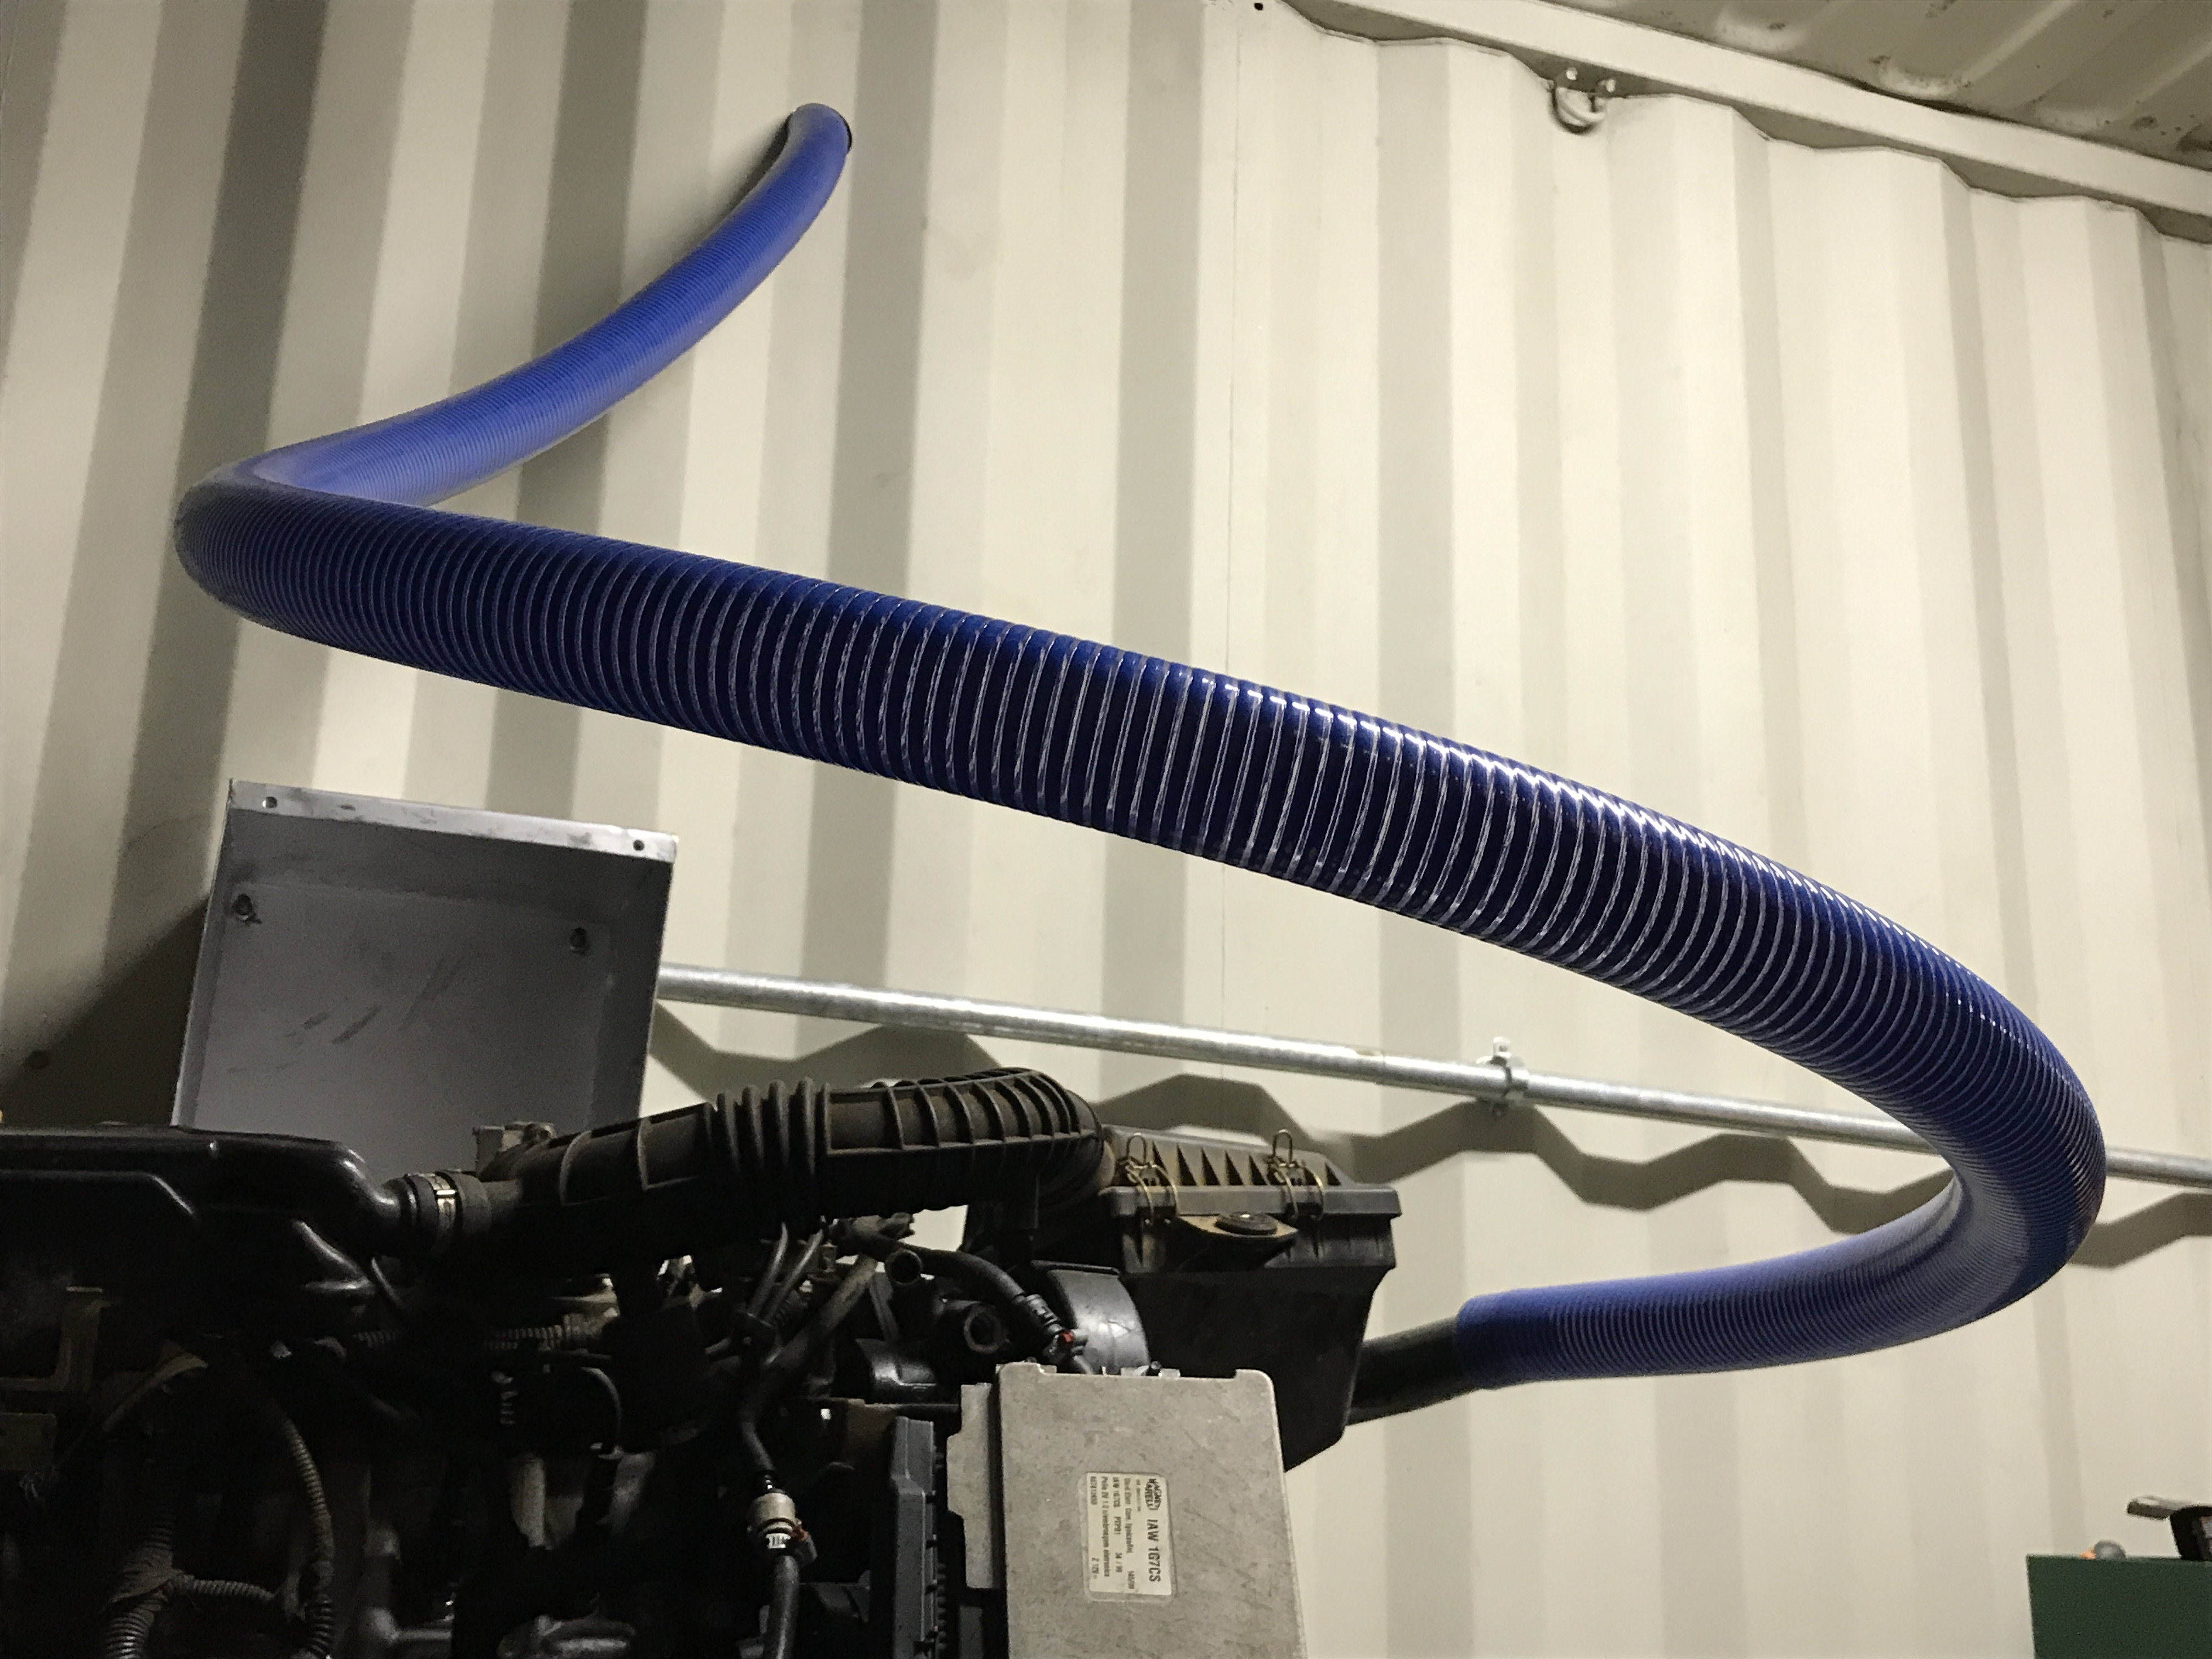
\includegraphics[keepaspectratio=true,scale= 0.09]{figuras/SistemaDeAdimissao.JPG}
	\caption{Mangueira do sistema de admissão}
	\label{mangueiraDoSistemaAdmissao}
\end{figure}

\begin{figure}[h!]
	\centering
	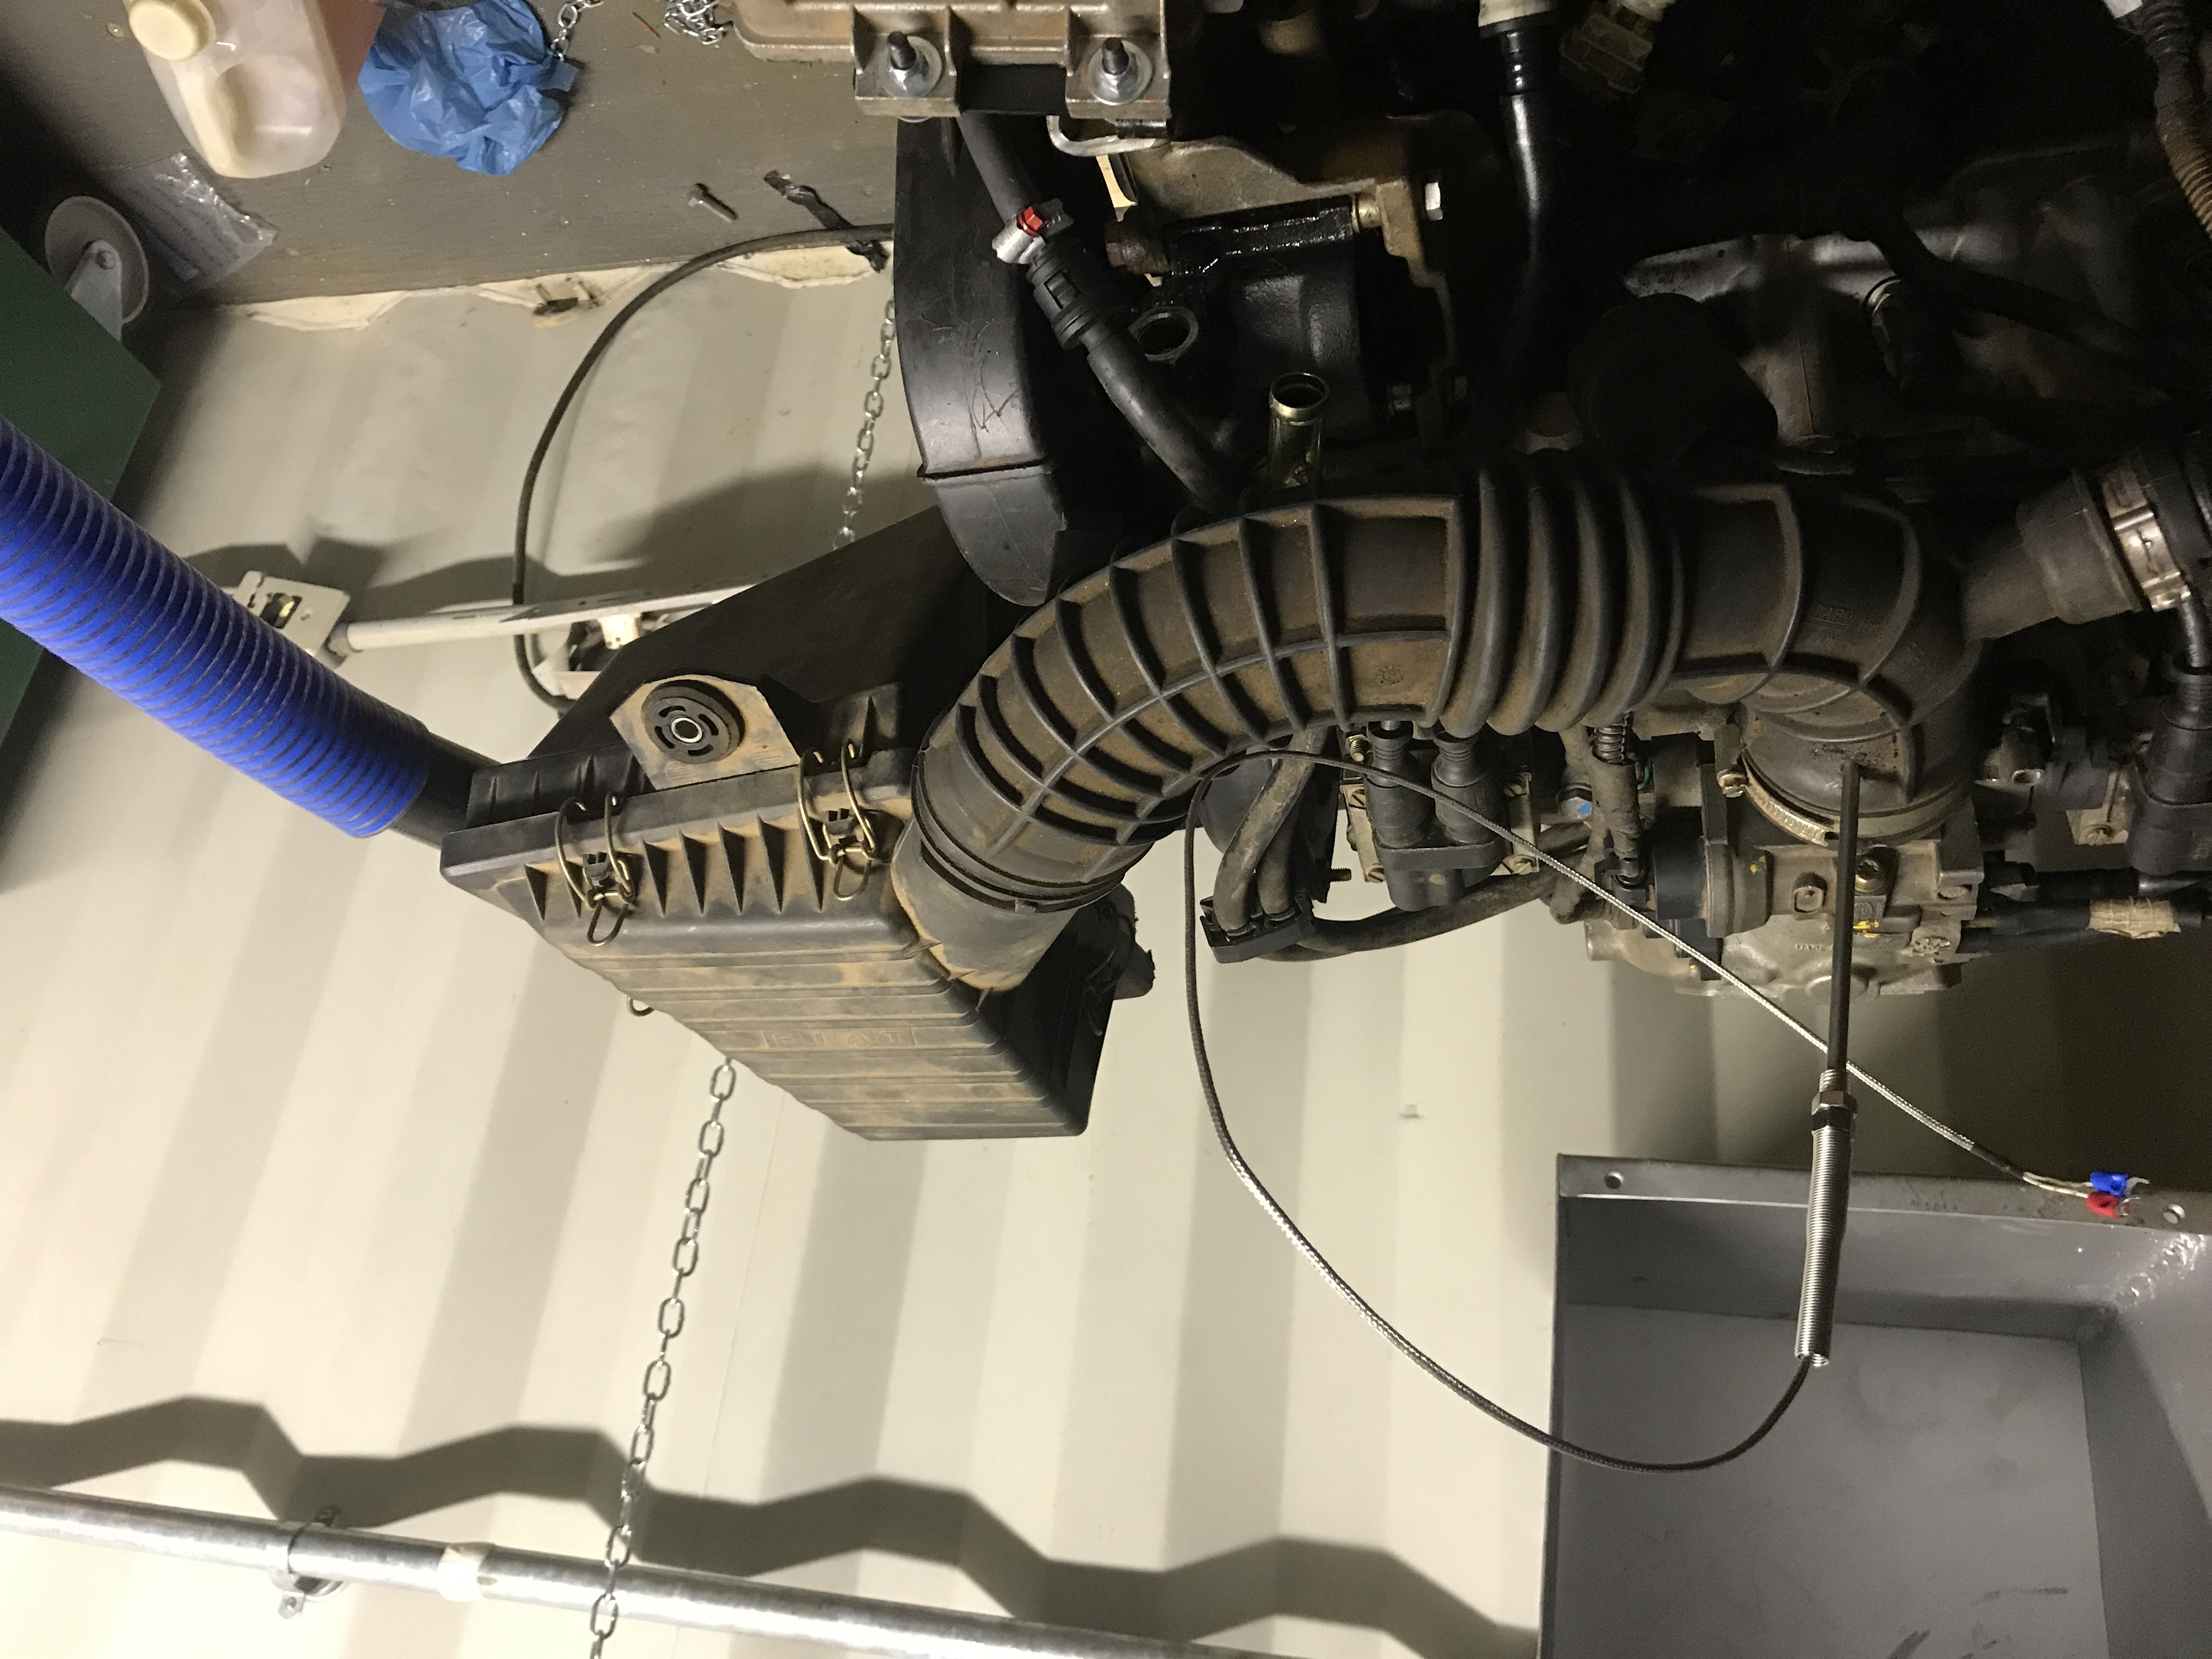
\includegraphics[keepaspectratio=true,scale= 0.09]{figuras/SensorDeTemperaturaNoSistemaDeAdmissao.JPG}
	\caption{Sensor de temperatura no sistema de admissão}
	\label{sensorDoSistemaAdmissao}
\end{figure}

\begin{figure}[h!]
	\centering
	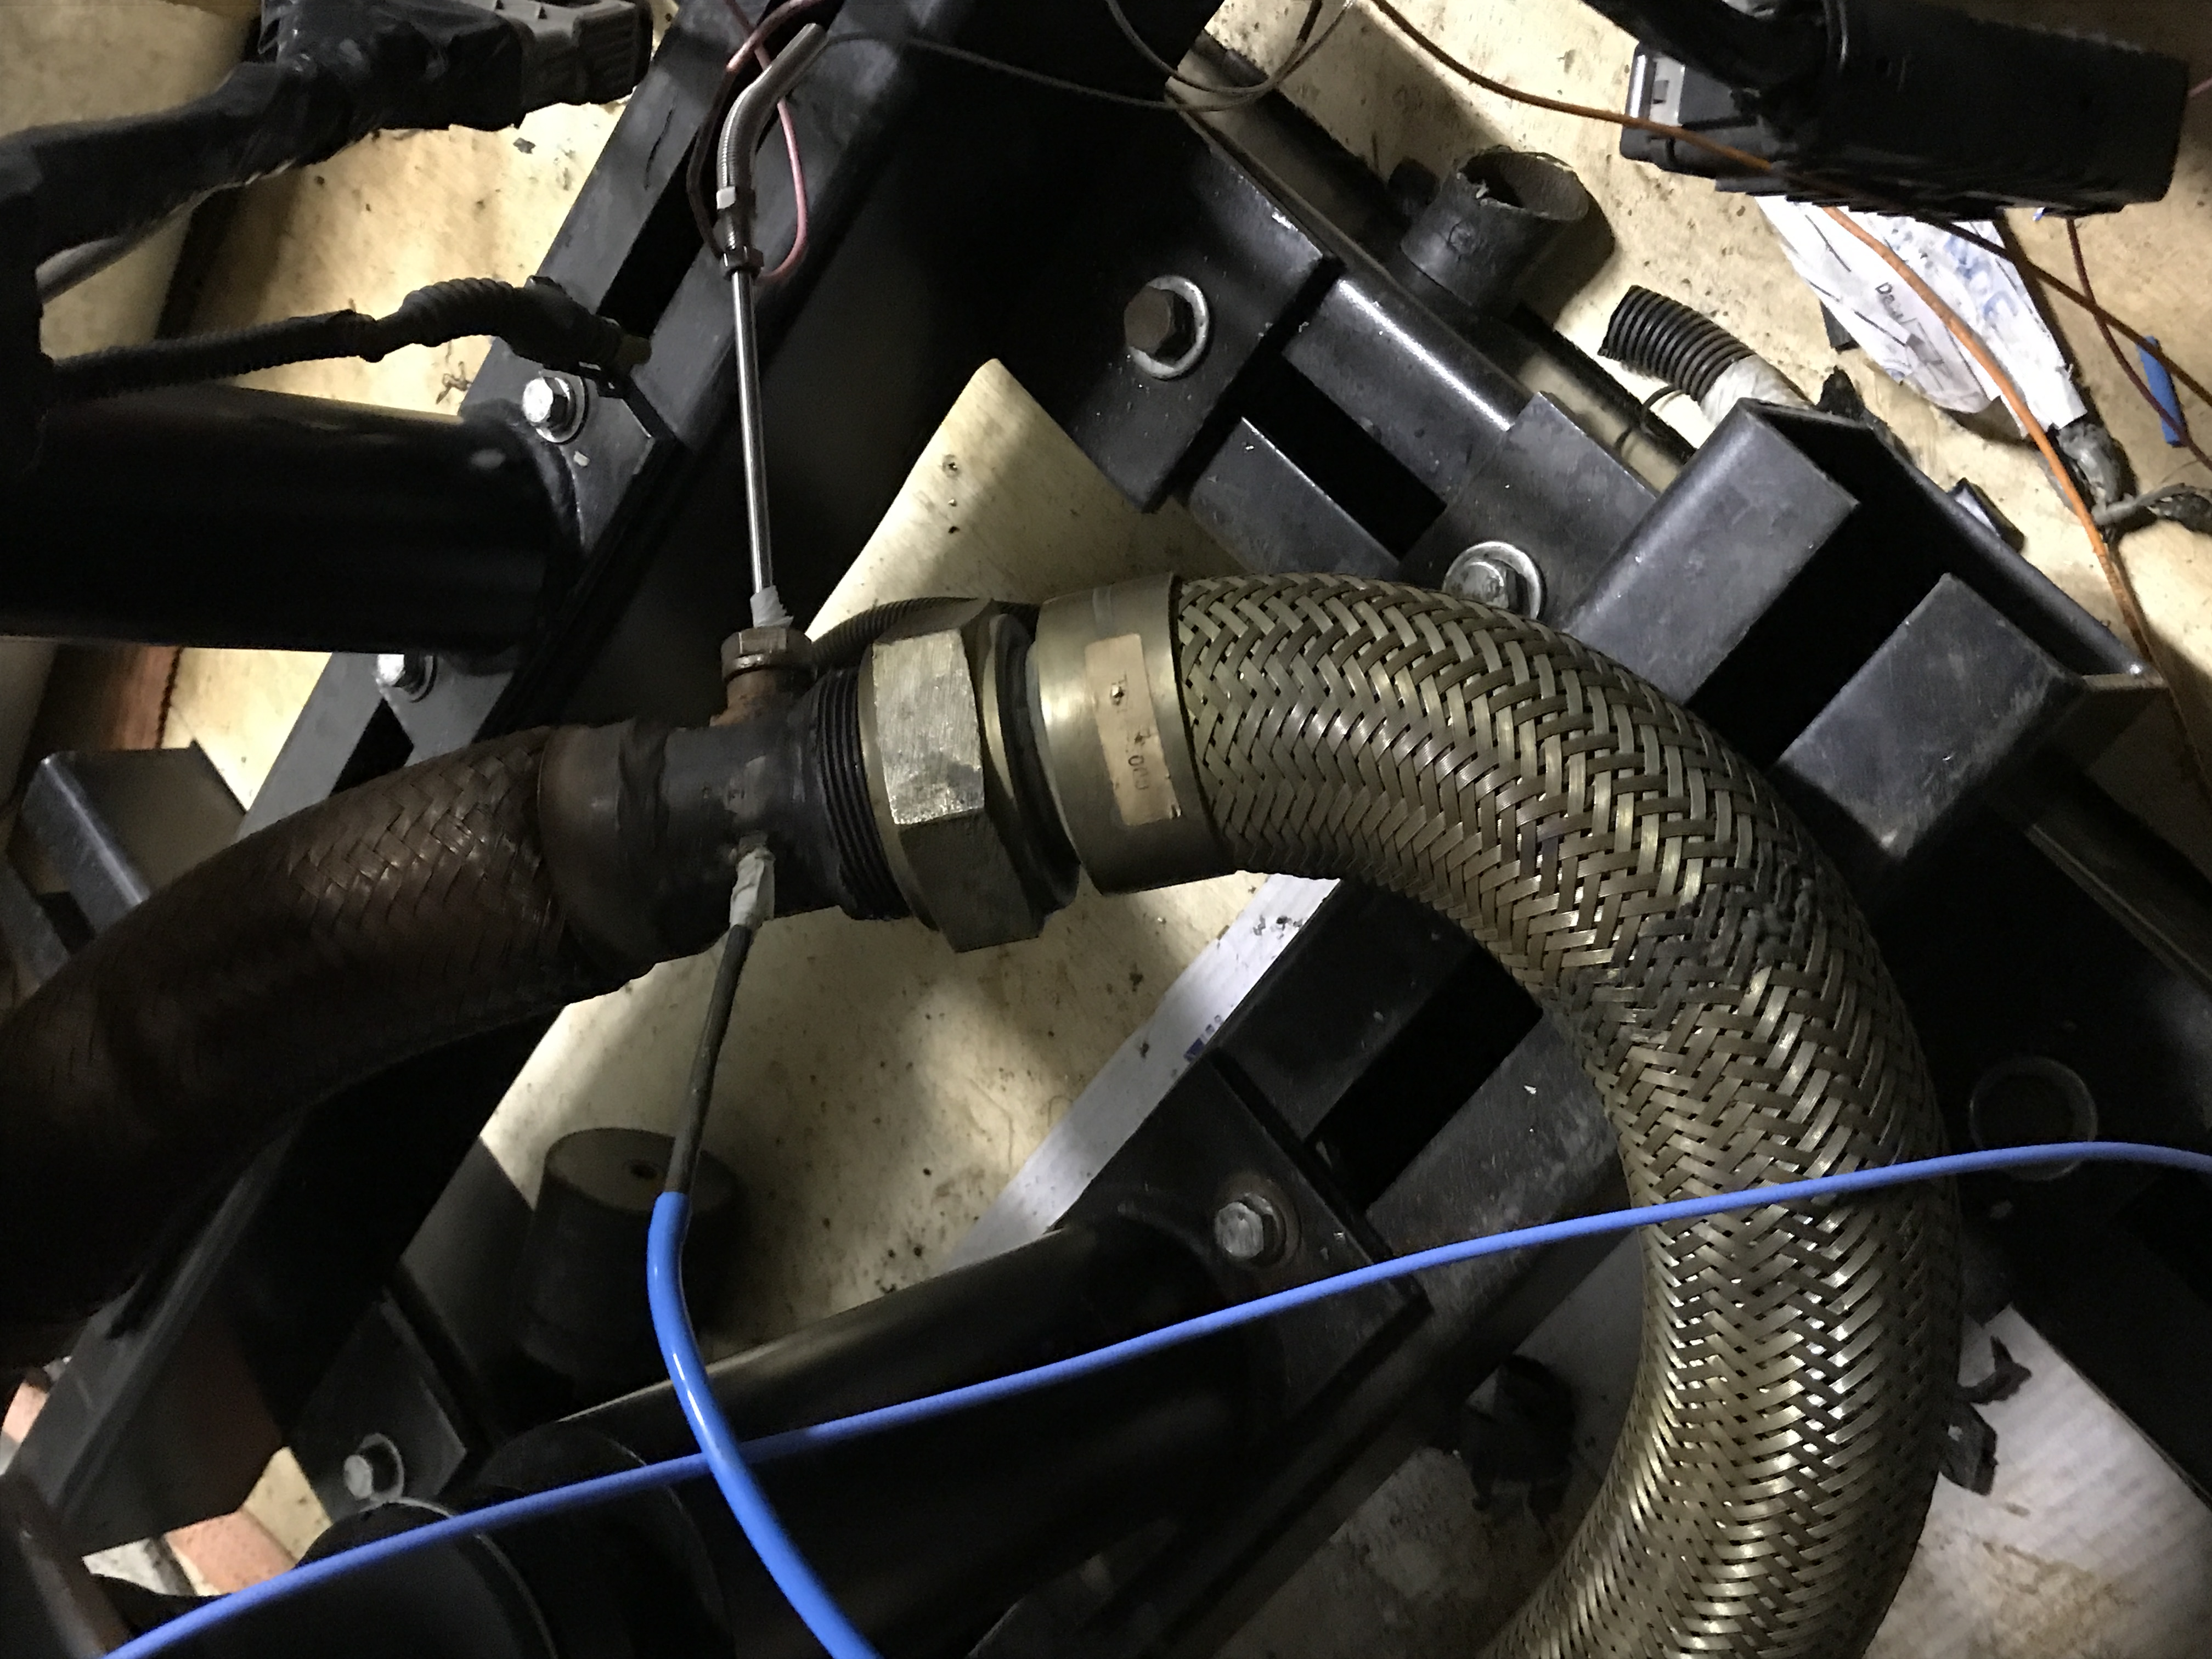
\includegraphics[angle=270,keepaspectratio=true,scale= 0.09]{figuras/SaidaParaSensorDePressaoETermopar.JPG}
	\caption{Saída para sensor de pressão e temopar}
	\label{saidaParaSensorDePressao}
\end{figure}
